% IEEE Signal Processing Letters
% SPL rules: technical content (title..conclusion, incl. figures/tables/proofs) <= 4 pages;
%            a 5th page is available for REFERENCES ONLY.
%            Abstract 100-175 words, no abbreviations/footnotes/displayed equations/references.
% EDICS: MSP-WAT (primary); MSP-SECU / MSP-FOR (secondary).
\documentclass[journal]{IEEEtran}
\usepackage[T1]{fontenc}
\usepackage{amsmath,amssymb}
\usepackage{graphicx}
\usepackage{booktabs}
\usepackage{url}
\usepackage{cite}

% ---- math macros ----
\newcommand{\sxi}{\sigma_\xi}
\newcommand{\sfwd}{\sigma_{\mathrm{fwd}}}
\newcommand{\Tf}{T_f}
\newcommand{\Lobs}{L_{\mathrm{obs}}}
\newcommand{\Ns}{N_s}
\newcommand{\ks}{k_s}
\newcommand{\Nmax}{N_{\max}}
\newcommand{\muY}{\mu_Y}
\newcommand{\pbit}{\varepsilon}
\newcommand{\Lh}{L_h}
\newcommand{\Prob}{\mathbb{P}}
\newcommand{\E}{\mathbb{E}}
\newcommand{\Bin}{\mathrm{Bin}}

\newtheorem{proposition}{Proposition}
\newtheorem{remark}{Remark}

\begin{document}

\title{Detection-Theoretic Sync-Header Design for IPD-QIM Timing Watermarks under Insertion--Deletion Channels}

\author{Jiuxiang~Cao,~Guang~Cheng,~and~Guangjie~Liu%
\thanks{This work was supported by the National Natural Science Foundation of China under Grant U2436601.}%
\thanks{J. Cao is with the School of Cyber Science and Engineering, Southeast University, Nanjing 211189, China, and also with Jinling Technology Group, Nanjing 210000, China (e-mail: caojiuxiang@seu.edu.cn).}%
\thanks{G. Cheng is with the School of Cyber Science and Engineering, Southeast University, Nanjing 211189, China (e-mail: chengguang@seu.edu.cn).}%
\thanks{G. Liu is with the School of Electronic and Information Engineering, Nanjing University of Information Science and Technology, Nanjing 210044, China (e-mail: gjieliu@nuist.edu.cn).}}

\maketitle

\begin{abstract}
Timing watermarks embedded by quantization index modulation on inter-packet delays can be demodulated only after their periodic frames are located, yet insertions and deletions repeatedly displace those frames: synchronization, not signal strength, is the binding constraint. Existing watermarks nonetheless fix sync-header parameters empirically, without a false-alarm budget. We cast periodic sync-header detection as a finite-window hypothesis test and select its parameters under a false-alarm budget. Under independent background bits, a Hamming-balanced header controls any common bit marginal, and a scan window no longer than the codeword region gives binomial domination for re-anchored tracks, yielding a certified false-alarm bound. The usual product over candidate tracks is provably optimistic, so we design against a scan statistic instead. The designs use 8--12-bit headers at corruption rates $0.2\%$--$5\%$ and meet a $10^{-9}$ budget, delivering a conservative decodable yield of $65$ down to $26$ frames that measurement exceeds throughout. Real Tor and VPN traces provide empirical false-hit measurements and guide header selection, without extending the analytical guarantee to dependent backgrounds. The result replaces trial-and-error tuning with budget-certified sync-header design.
\end{abstract}

\begin{IEEEkeywords}
Timing watermarking, quantization index modulation, insertion--deletion channel, frame synchronization, detection theory, false alarm.
\end{IEEEkeywords}

\IEEEpeerreviewmaketitle

\section{Introduction}
\label{sec:intro}
Timing watermarking embeds a recoverable identifier by perturbing inter-packet delays (IPDs), and is the standard way to link flows across multi-hop encrypted links, where payload and packet size carry no usable signal \cite{Wang2003Stepping,Li2026Survey}. The embedder of choice is quantization index modulation (QIM) \cite{ChenWornell2001QIM}: each IPD is quantized to an interleaved lattice selected by a watermark bit, and the detector hard-decides the received IPDs against those lattices. Demodulation presupposes knowing where each frame begins---exactly what the channel destroys. Packets are inserted and deleted by congestion loss, retransmission, keep-alive traffic and re-segmentation \cite{Paxson1999E2E,Bennett1999Reorder}, by an adversary breaking the mark \cite{Lin2012}, or by defenses that reshape the IPDs to erase it \cite{Yuan2025DeMarking}; each event displaces every subsequent symbol index. The impairment is a \emph{synchronization} error, not additive noise, and enlarging the quantization step cannot trade it away: once the frame drifts uncorrected, a fixed read position returns misaligned symbols. Even the simplest deletion channel has no closed-form capacity \cite{Mitzenmacher2009Survey}.

The remedy is a known sync header repeated in every frame and re-located by correlation---the mechanism behind marker and watermark codes for insertion--deletion channels \cite{DaveyMacKay2001}. The detector scans offsets about the predicted phase, declares a hit when the correlation exceeds a threshold and presence only after several hits accumulate along a periodic track. Anchoring is thus a detection problem in its own right.

Existing designs---error correction over substitution/deletion/insertion channels \cite{Gong2013Invisible}, exploiting the network's reaction to loss \cite{Iacovazzi2018DropWat}, heterogeneous time channels \cite{Li2022HeteroTiC}, packet-count modulation \cite{Qiao2025DynMark}, or packet order with timing \cite{Feng2024HSTW}---fix the detector parameters empirically, without solving them against $\lambda$ under a false-alarm budget. The sync-header length $\Lh$, threshold $\tau$, radius $R$ and confirmation count are coupled through $\lambda$, and $\Lh$ is squeezed from two sides: a long header forms a peak only if no edit falls inside it, an event of probability $(1-\lambda)^{\Lh}$, while a short one is imitated by chance and the $\pm R$ scan lifts the false-hit floor by roughly the window size.

This letter casts sync-header detection as a finite-window hypothesis test. Under independent background bits, Hamming balance controls arbitrary common marginals (Prop.~\ref{thm:balance}) and $2R\le L_c$ yields binomial domination despite re-anchoring (Prop.~\ref{thm:fa}); the optimistic product over candidate tracks is replaced by a nominal scan statistic (Prop.~\ref{thm:fkg}). Spectral alignment diagnoses background dependence empirically on Tor and VPN traces; synthetic flows test tracking yields.

\section{Signal Model and Detection Problem}
\label{sec:model}
A marked flow traverses a $K$-hop encrypted link; the detector observes only receive-side timing and must decide whether the flow carries a watermark, recovering the local phase of the periodic sync header in the process. We write $\Bin(n,p)$ for the binomial law.

\subsection{Embedding and per-symbol reliability}
The causal QIM embedder (delay-only) quantizes each output IPD to an interleaved lattice selected by the watermark bit, with step $\Delta$; the detector returns $\hat b=\mathrm{round}(2x/\Delta)\bmod 2$ from a received IPD $x$. After $K$ hops the timing noise is the difference of adjacent-packet jitters, $\sxi=\sqrt{2K}\,\sfwd$ with per-hop jitter spread $\sfwd$, and the per-symbol error rate is exactly the \emph{folded} tail
\begin{equation}
\pbit=\Prob[\,\mathrm{round}(2\xi/\Delta)\ \text{odd}\,],
\label{eq:eps}
\end{equation}
whose first term is the familiar $2Q(\Delta/4\sxi)$. We take $\pbit=5\%$ ($\Delta/\sxi\approx7.8$ under Gaussian jitter). Sec.~\ref{sec:num} shows \eqref{eq:eps} is insensitive to the jitter law there, so $\pbit$ is an exogenous design input.

\subsection{Periodic frame and windowed correlation detector}
The watermark occupies period-$\Tf$ frames, each a known length-$\Lh$ bipolar sync header $g\in\{\pm1\}^{\Lh}$ followed by a length-$L_c=\Tf-\Lh$ codeword region of coded random bits, which synchronization ignores. The detector scans $W:=2R+1$ offsets within $\pm R$ of the predicted phase, forming the matched-bit count $C(j)$ between $g$ and the hard-decided receive bits. Any $C(j)\ge\tau$ is a hit, re-anchoring the next frame at the top-scoring offset (leftmost on ties); otherwise the phase advances by $\Tf$, so a missed sync header costs one confirmation, not the track. We design anchoring and presence detection only, not codeword decoding.

\subsection{Insertion--deletion channel and lock maintenance}
A dropped packet merges its two flanking IPDs into one longer gap (a deletion, $2\to1$); a retransmission, keep-alive, re-segmentation or cover packet splits one IPD into two (an insertion, $1\to2$). Each IPD position independently deletes with probability $\lambda_d$, inserts with probability $\lambda_i$, and is otherwise kept, $\lambda=\lambda_d+\lambda_i$ (symmetric baseline $\lambda_i=\lambda_d=\lambda/2$). A deletion fuses two symbols into one of effectively random value, an insertion splits one into two random ones; the net drift is $\mp1$, matching the standard insertion--deletion count \cite{Mitzenmacher2009Survey}. Realistic $\lambda$ is $[0.5\%,2\%]$ on broadband links, higher when congested \cite{Paxson1999E2E,Bennett1999Reorder}; Sec.~\ref{sec:num} reports the cost of bursty and asymmetric departures.

An edit inside the sync header misaligns it and collapses the correlation peak; an edit outside merely shifts the phase. Between re-anchors the drift $\Delta_{\mathrm{frame}}$ is a random walk with mean $(\lambda_i-\lambda_d)\Tf$ and variance $\Tf[\lambda-(\lambda_i-\lambda_d)^2]$, which at the symmetric baseline is zero-mean with variance $\lambda\Tf$; the frame stays anchorable while $|\Delta_{\mathrm{frame}}|\le R$. Lock must hold over a whole track, so with $P_{\mathrm{out}}:=\Prob(|\Delta_{\mathrm{frame}}|>R)$ and $P_{\mathrm{in}}:=1-P_{\mathrm{out}}$ we size $R$ as the smallest radius with $1-P_{\mathrm{in}}^{\Nmax}\le\eta_{\mathrm{lock}}$ over the window's $\Nmax$ frames.

\section{Per-Slot Statistics and the Sync Header}
\label{sec:analysis}
\begin{table*}[t]
\centering\footnotesize
\setlength{\tabcolsep}{4.2pt}
\caption{Designs and tracking yields ($\pbit{=}5\%$, $L_c{=}10$, $\Lobs{=}2000$ IPDs); burst columns use length $20$.}
\label{tab:main}
\begin{tabular}{@{}c ccccccccc c ccccc@{}}
\toprule
& \multicolumn{9}{c}{design} & & \multicolumn{5}{c}{validation} \\
\cmidrule(r){2-10}\cmidrule(l){12-16}
$\lambda$(\%) & $\Lh$ & $\tau$ & $R$ & $\Ns$ & $\ks$ & $q/p_W$ & $\Nmax$ & $P_{\mathrm{D}}$ & $\muY^{\mathrm{dec}}$ & & $Y_{\mathrm{hit}}$ & $Y_{\mathrm{exact}}$ & $Y_{\mathrm{exact}}/Y_{\mathrm{hit}}$ & blackout & $Y_{\mathrm{exact}}$ burst \\
\midrule
0.2 & 10 & 9 & 2 & 18 & 15 & 17 & 100 & 0.994 & 65 & & 89.1 & 88.7 & 0.995 & 0.10 & 85.7 \\
0.5 & 10 & 9 & 3 & 26 & 20 & 12 & 100 & 0.991 & 63 & & 89.2 & 87.2 & 0.977 & 0.13 & 83.3 \\
1 & 10 & 9 & 3 & 31 & 22 & 11 & 100 & 0.990 & 60 & & 82.9 & 79.1 & 0.954 & 0.27 & 77.2 \\
2 & 8 & 8 & 4 & 42 & 19 & 16 & 111 & 0.993 & 45 & & 62.3 & 60.3 & 0.968 & 0.36 & 58.5 \\
3 & 8 & 8 & 5 & 74 & 27 & 12 & 111 & 0.991 & 42 & & 56.0 & 47.9 & 0.855 & 0.39 & 56.5 \\
4 & 12 & 11 & 5 & 58 & 22 & 15 & 90 & 0.991 & 35 & & 54.9 & 47.3 & 0.861 & 0.38 & 59.6 \\
5 & 10 & 10 & 5 & 58 & 14 & 33 & 100 & 0.991 & 26 & & 35.1 & 31.9 & 0.911 & 0.55 & 40.9 \\
\bottomrule
\end{tabular}
\end{table*}

Fix $(\Lh,\tau,R)$. The elementary question is whether one frame slot is declared a hit: under $H_1$ this requires the sync header to survive the channel, the correlation to clear the threshold, and the drift to lie inside the scan window.

\begin{proposition}[Per-slot rates and efficient anchoring]
\label{thm:hit}
Let $p_0$ be the single-offset false-hit rate, $p_W$ the rate with the $\pm R$ scan, and $q:=(1-\lambda)^{\Lh}P_\tau P_{\mathrm{in}}$ with $P_\tau=\Prob[\Bin(\Lh,\pbit)\le \Lh-\tau]$. Then
\begin{equation}
p_W\le W p_0,\qquad q_1=q+\big[1-(1-\lambda)^{\Lh}\big]p_W,
\label{eq:qp0}
\end{equation}
the first inequality holding for any dependence between offsets; the separation constraint $q\ge10\,p_W$ of Sec.~\ref{sec:num} keeps $q_1\approx q$, so $q$ is used throughout. For full match $\tau=\Lh$, $P_{\mathrm{in}}\approx1$ and to first order in $p_0$, clean hits dominate the background floor exactly when
\begin{equation}
\beta\,\Lh>\ln(2R+1),\qquad \beta:=\ln[2(1-\lambda)(1-\pbit)] .
\label{eq:info}
\end{equation}
\end{proposition}
\begin{IEEEproof}
$p_W\le Wp_0$ is the union bound over the $W$ offsets. A clean hit needs three simultaneous events---sync header free of internal edits ($(1-\lambda)^{\Lh}$), drift inside the window ($P_{\mathrm{in}}$), threshold pass ($P_\tau$)---whose product is $q$; a header struck internally degrades to $p_W$. For $\tau=\Lh$ and fair bits, $p_0=2^{-\Lh}$ and $P_\tau=(1-\pbit)^{\Lh}$, so $q>p_W$ reads $[2(1-\lambda)(1-\pbit)]^{\Lh}>2R+1$.
\end{IEEEproof}

Condition \eqref{eq:info} is the feasibility condition: long headers are penalized through $(1-\lambda)^{\Lh}$, short ones through $\ln(2R+1)$, and since $R$ grows with $\lambda$ the feasible band of $\Lh$ narrows as $\lambda$ rises.

\subsection{The sync header must be balanced}
Prop.~\ref{thm:hit} used $p_0=2^{-\Lh}$, i.e.\ that the hard-decided bits of unmarked traffic are fair. Real traffic violates this badly (Sec.~\ref{sec:num}); the following removes the assumption.

\begin{proposition}[Balanced sync header]
\label{thm:balance}
Let the background bits be independent with an arbitrary common marginal $\pi=\Prob(b=1)$, and let $g$ have Hamming weight $w$. Then
\begin{equation}
\E[C]=(\Lh-w)+(2w-\Lh)\pi,\quad \mathrm{Var}(C)=\Lh\,\pi(1-\pi),
\label{eq:balmean}
\end{equation}
so $\E[C]$ is free of $\pi$ if and only if $w=\Lh/2$, in which case $\E[C]=\Lh/2$ and, for every $\pi$ and every $\tau>\Lh/2$,
\begin{equation}
\Prob[C\ge\tau]\ \le\ \exp\!\big[-2(\tau-\Lh/2)^2/\Lh\big].
\label{eq:balance}
\end{equation}
\end{proposition}
\begin{IEEEproof}
Linearity gives $\E[C]=w\pi+(\Lh-w)(1-\pi)$; independence gives the variance in \eqref{eq:balmean}. The mean is constant exactly when $w=\Lh/2$. Then $C$ sums $\Lh$ independent indicators with total mean $\Lh/2$, so Hoeffding gives \eqref{eq:balance}.
\end{IEEEproof}

\begin{figure}[!t]
\centering
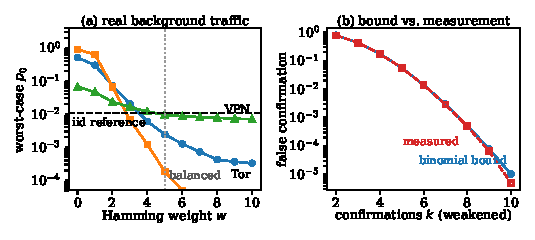
\includegraphics[width=\columnwidth]{figs/fig_balance_ladder.pdf}
\caption{Real-background false hits and the iid single-track binomial tail.}
\label{fig:balance}
\end{figure}

For Table~\ref{tab:main}'s thresholds $\tau=\Lh,\Lh-1$, put $m=\Lh/2$ and $v=\pi(1-\pi)$. The exact tails $v^m$ and $v^{m-1}[m-(2m-1)v]$ increase on $[0,1/4]$ for $m\ge2$, giving the uniform iid bound $p_0=\Prob[\Bin(\Lh,\tfrac12)\ge\tau]$. Odd lengths cannot balance and exceed this value by $4$--$8\%$ on the numerical grid; the search uses even $\Lh$.

Sec.~\ref{sec:num} reports unbalanced headers exceeding the independent-bit reference by up to $48\times$ on real traffic, and quantifies the residual excess for balanced headers.


Balance fixes the mean but not the variance under dependent bits. With background autocovariance $\gamma_k$ and aperiodic autocorrelation $c_k(g)=\sum_i g_ig_{i+k}$,
\begin{equation}
4\,\mathrm{Var}(C)=\gamma_0\Lh+2\textstyle\sum_{k\ge1}\gamma_k\,c_k(g)=:V(g).
\label{eq:align}
\end{equation}
Signed covariance contributions are not determined by sidelobe magnitudes alone. Selection in Sec.~\ref{sec:num} is empirical; variance control gives no dependent-background tail guarantee.

\section{Certified Error Probabilities and Constrained Design}
\label{sec:design}
\subsection{A certified false-alarm bound}
A track confirms on its $k$th hit within $N$ slots including capture. Blind capture tests every complete header; scans consider only complete headers, break ties leftmost and terminate when none remains. The rejection window $\Lobs$ counts received IPDs ($\Lobs+1$ packets). Re-anchoring changes the nominal span $S(N)=(N-1)\Tf+\Lh$; the detection model admits $J=\max\{0,\lfloor(\Lobs-S(N)+1)/\Tf\rfloor\}$ full-track starts.

\begin{proposition}[Certified false alarm]
\label{thm:fa}
Assume independent background bits with a common marginal, a balanced header, $2\le k\le N$, a valid single-offset bound $p_0$, and
\begin{equation}
2R\le L_c.
\label{eq:disjoint}
\end{equation}
Set $n=N-1$, $r=k-1$, $u=\min\{1,Wp_0\}$, and $B_n=\Prob[\Bin(n,u)\ge r]$. Then
\begin{equation}
P_{\mathrm{FA}}(N,k;\Lobs)\ \le\ M_{\rm eff}\,p_0 B_n,
\label{eq:fa}
\end{equation}
where $[x]_+=\max\{0,x\}$, $w_t=[\Lobs-\Lh-t\Tf+rR+1]_+$ and
\[
M_{\rm eff}=B_n^{-1}\sum_{t=r}^{n}w_t\binom{t-1}{r-1}u^r(1-u)^{t-r}.
\]
Set $M_{\rm eff}=0$ if $B_n=0$; endpoint weights are extended by continuity.
\end{proposition}
\begin{IEEEproof}
Fix a start $s$, not conditioned on blind selection, and reveal only its track. Anchors advance by at least $\Tf-R\ge\Lh$ per slot, so scan right endpoints increase; after a miss, the next scan starts $\Tf-2R-\Lh+1\ge1$ beyond the previous endpoint. Capture likewise precedes its first scan. Conditional on any initial-header realization, each hit run therefore starts on fresh bits. Fixing $\ell$ hit offsets specifies disjoint headers separated by at least $\Tf-R\ge\Lh$. Dropping score-competition conditions and summing $W^\ell$ offset strings bounds the conditional run tail by $u^\ell$.

A conditional quantile coupling (Skorokhod representation) bounds these runs by independent geometric runs with tail $u^\ell$. Actual misses occur no later than reference misses, so hits in the first $m$ subsequent slots are dominated by $\Bin(m,u)$. This holds with clipped scans and zero-padding after termination; $u=0,1$ use constant reference sequences.

The $r$th subsequent hit at slot $t$ starts at least at $s+t\Tf-rR$. Completeness forces $t\le m_s=\min\{n,\lfloor(\Lobs-\Lh-s+rR)/\Tf\rfloor\}$, bounding the $r$th-hit time, not the executed slots. Thus confirmation from $s$ has probability at most $p_0\Prob[\Bin(m_s,u)\ge r]$, zero for $m_s<r$. Expanding this reference tail by its $r$th-success time and summing over $s$ gives the weight $w_t$ and \eqref{eq:fa}.
\end{IEEEproof}

Condition \eqref{eq:disjoint} ensures fresh scans after misses, not independent slots; $M_{\rm eff}$ accounts for re-anchoring and finite-window completion.

\subsection{Detection: the product form is optimistic}
The detection side cannot be repaired the same way: it errs in the opposite direction.

\begin{proposition}[Detection is over-counted]
\label{thm:fkg}
In the nominal model, take independent $H_i\sim\Bin(1,q)$ and $\mathrm{cap}_i\sim\Bin(1,q_{\rm cap})$, $1\le i\le\Nmax$, with blind-capture rate $q_{\rm cap}=(1-\lambda)^{\Lh}P_\tau$. For $p_{\mathrm{tr}}=q_{\rm cap}\Prob[\Bin(N-1,q)\ge k-1]$,
\begin{equation}
P_{\mathrm{D}}(N,k;\Lobs)\ \le\ 1-(1-p_{\mathrm{tr}})^{J}.
\label{eq:pd}
\end{equation}
\end{proposition}
\begin{IEEEproof}
All tracks share these coordinates. Their confirmation events $A_f=\{\mathrm{cap}_f=1,\ \sum_{i=f+1}^{f+N-1}H_i\ge k-1\}$, $1\le f\le\min\{J,\Nmax-N+1\}$, are increasing events of probability $p_{\mathrm{tr}}$ each. Harris/FKG gives $\Prob[\bigcap_f A_f^c]\ge\prod_f\Prob[A_f^c]\ge(1-p_{\mathrm{tr}})^J$, proving \eqref{eq:pd}.
\end{IEEEproof}

Thus \eqref{eq:pd} is a search relaxation, not a detection guarantee: it accepts a $\lambda=5\%$ candidate whose nominal scan estimate is $0.960$. We estimate $\Prob[\bigcup_f A_f]$ with $8\times10^4$ replicates (standard error below $4\times10^{-4}$), prefiltered by \eqref{eq:pd}.

\subsection{Constrained design}
With $\Tf=\Lh+L_c$ and $\Nmax=\lfloor \Lobs/\Tf\rfloor$, the aligned frames delivered are $Y\sim\Bin(\Nmax,q)$, and $\muY=\Nmax(1-m_q)q$ is the conservative yield. The search rule takes the shortest track $(\Ns,\ks)$, $\ks\ge2$, for each even $\Lh$ and $\tau$, meeting the certified \eqref{eq:fa} at level $\alpha$ and the scan-statistic constraint $P_{\mathrm D}\ge1-\delta$ subject to $\Ns\Tf\le\Lobs$ and \eqref{eq:disjoint}, then maximizes:
\begin{equation}
(\Lh^\ast,\tau^\ast)=\arg\!\max_{(\Lh,\tau)\ \text{feasible}}\ \muY,\quad q=(1-\lambda)^{\Lh}P_\tau P_{\mathrm{in}}.
\label{eq:design}
\end{equation}
Margins $m_q$ on $q$ and $f_{\mathrm{fa}}$ on $p_0$ are applied before every budget check. The latter is an empirical allowance informed by Sec.~\ref{sec:num}, not a guarantee for dependent backgrounds.

\section{Numerical Results and Validation}
\label{sec:num}
\subsection{Configuration and design}
We take $\pbit=5\%$, $L_c=10$, $\alpha=10^{-9}$, $1-\delta=0.99$, $\Lobs=2000$ received IPDs ($2001$ packets, $\approx20$~s at $10$~ms mean spacing), $\eta_{\mathrm{lock}}=10^{-3}$, $m_q=0.15$ and $f_{\mathrm{fa}}=2$. The search sizes $R$ by cumulative lock and enumerates even $\Lh$ and $\tau$ for \eqref{eq:design}. The configurations in Table~\ref{tab:main} remain feasible under \eqref{eq:fa} (max $9.662\times10^{-10}$); shortest-track optimality is not claimed. The search finds none at $\lambda=6\%$.

Dropping the constraint $q\ge10\,p_W$ is instructive: the search then prefers very short sync headers ($\Lh=6$ at $\lambda=0.5\%$) and the nominal yield rises by up to $15\%$, but $p_W\approx0.11$ there, and a chance full match inside the codeword region falls within the $\pm R$ window and \emph{steals the anchor}---an effect the per-slot model does not capture. Over ten balanced sync headers the decodable yield spans $75.4$--$88.1$ frames, the worst reaching $\muY$ itself; under the margin, $83.9$--$87.0$. Here, unlike in Sec.~\ref{sec:analysis}, sidelobe magnitude matters.

\subsection{Real background traffic}
The false-alarm analysis stands or falls on the hard-decided bits of unmarked traffic. We test it on per-packet IPD pools from the ISCXTor2016 and ISCXVPN2016 captures \cite{Lashkari2017Tor,Draper2016VPN} ($9.2\times10^6$ Tor and $1.9\times10^6$ VPN delays, grouped by application), hard-decided by the rule of Sec.~\ref{sec:model}.

The bits are far from fair: at $\Delta=19$~ms the marginal ranges over $0.05$--$0.33$ across application classes, with lag-one autocorrelation up to $+0.24$. Averaging over sync headers hides this, but the rate is strongly \emph{header}-dependent (Fig.~\ref{fig:balance}(a)): $p_0$ falls monotonically with Hamming weight, from $0.51$ for the all-zero header ($48\times$ the bound) to $0.0024$ for a balanced one. Over the \emph{complete} balanced class ($252$ headers at $\Lh=10$, $924$ at $\Lh=12$) and $24$ cells (four pools, three $\Delta$, both even-length configurations) the worst ratio to the fair-bit $p_0$ is $1.14$ and most fall below~$1$. These are empirical comparisons with the independent-bit reference; the nearest-to-balanced headers of odd $\Lh=11$ reach $2.2\times$.

Dependence is the residual. Over $144$ cells at the configurations of Table~\ref{tab:main}, seven exceed the bound by more than $1.5\times$, six from one cell---Tor file transfer at $\Delta=1$~ms, whose bit stream keeps a period-three structure at mild bias---reaching $7.7\times$. Neither the background autocorrelation nor the header's sidelobe magnitude predicts which headers fail there (Spearman $-0.12$); the covariance-weighted alignment $V(g)$ of \eqref{eq:align} does ($+0.75$, $+0.85$), and for $(\Lh,\tau)=(10,10)$ the lowest-$V(g)$ decile reduces the worst ratio from $7.7$ to $0.18$ on the same sample. This selection diagnostic gives no dependent-traffic guarantee; $f_{\mathrm{fa}}=2$ covers every measured cell but that one.

\subsection{Is the certified bound reachable?}
The $10^{-9}$ certificate is analytical. At $\lambda=2\%$, the scan bound $p_W\le Wp_0$ is $0.0352$ versus $0.0349$ measured. Weakening $k$ over $2\times10^5$ iid-background tracks gives false-confirmation rates $0.77$--$5\times10^{-6}$; the single-track binomial-tail/measurement ratio is $[1.00,2.07]$, apart from one value below unity within Monte-Carlo error (Fig.~\ref{fig:balance}(b)). This tests accessible rates, not independence or the $10^{-9}$ target.

\subsection{Delivered frames, bursts, asymmetry, jitter}
Yield experiments start from the channel-mapped first-frame anchor, measuring tracking rather than blind confirmation. Separating hits by anchor error shows that the aligned-frame count $Y_{\mathrm{hit}}$ over-counts: $0.5\%$--$14.5\%$ of ``aligned'' frames sit at a non-zero offset or at a multiple of $\Tf$---a \emph{frame-index slip}, where periodic lock survives but the frame number does not. We therefore report the decodable yield $\muY^{\mathrm{dec}}=\rho\muY$ with a measured anchor-exactness factor $\rho=0.85$, which the exactly indexed $Y_{\mathrm{exact}}$ exceeds in every row by $14\%$ or more; that $\rho$ is measured, not predicted, is a limitation of the model.

\emph{Bursts.} Under Gilbert--Elliott edits at matched mean $\lambda$, with the parameters of Table~\ref{tab:main} unchanged, the correlation peak does not collapse: at $\lambda\ge4\%$ clustering leaves more sync headers wholly intact and the per-slot rate \emph{rises} ($q$ from $0.368$ to $0.430$ at $\lambda=5\%$). What degrades is continuity: the fraction of tracks with eight or more consecutive missed slots grows with burst length at every $\lambda\le4\%$, from $0.00$--$0.10$ under independent edits to $0.10$--$0.39$ at mean burst length $20$ (Table~\ref{tab:main}).

\emph{Re-capture.} That motivates re-acquisition, but the obvious rule fails: widening the scan to $3R$ after four consecutive misses, compared on identical channel realisations over $800$ flows, gains $+4.4\pm0.8$ frames at $\lambda=1\%$ but loses $-3.6\pm1.1$ at $3\%$ and $-2.6\pm0.8$ at $5\%$. Raw hits rise while correctly indexed frames fall: a wider window buys wrong-offset anchors faster than it recovers true ones, and a full-match requirement does not help. Recovering a lost track needs the frame \emph{index} re-established, not the phase.

\emph{Asymmetry and jitter.} With $(\lambda_i-\lambda_d)/\lambda=0.5$ the designs at $\lambda=2\%$ and $3\%$ are unchanged; the cost is certifiability, not lock loss, since $R$ grows by one and can break \eqref{eq:disjoint} ($\lambda=5\%$ then needs $L_c=14$, $\muY$ falling to $20$). Finally, \eqref{eq:eps} is insensitive to the jitter law at $\Delta/\sxi=7.8$ ($\pbit=0.027$--$0.055$ across Gaussian, Laplace, Student-$t_3$, lognormal and Pareto); heavy tails matter only asymptotically, putting a floor under $\pbit$ that no quantization step removes ($0.0001$ against $0.0036$ for $t_3$ at $\Delta/\sxi=16$).

\emph{Latency.} Screening $L_1=400$--$800$ IPDs with iid false-alarm bound $\overline P_{\mathrm{FA},1}$ gives rejection-latency upper bounds of $418$--$871$ IPDs; \eqref{eq:fa} still bounds false alarm, and detection may decrease.


\section{Conclusion}
\label{sec:conclusion}
Sync-header selection under insertion--deletion admits a finite-window false-alarm certificate for independent background bits with a common marginal, balanced headers and $2R\le L_c$. Detection is a nominal scan statistic; the tested real traffic gives empirical evidence, not a certificate for dependent backgrounds. Code and results: \url{https://github.com/gjieliu/spl-sync-header-design}.

\bibliographystyle{IEEEtran}
\bibliography{references}

\end{document}
